%%%%%%%%%%%%%%%%%%%%%%%%%%%%%%%%%%%%%%%%%%%%%%%%%%%%%%%%%%%%%%%%%%%%%%%%%%%%
%%%%%%%%%%%%%%%%%%%%%%%%%%%%%%%%%%%%%%%%%%%%%%%%%%%%%%%%%%%%%%%%%%%%%%%%%%%%
% Article
%%%%%%%%%%%%%%%%%%%%%%%%%%%%%%%%%%%%%%%%%%%%%%%%%%%%%%%%%%%%%%%%%%%%%%%%%%%%
%%%%%%%%%%%%%%%%%%%%%%%%%%%%%%%%%%%%%%%%%%%%%%%%%%%%%%%%%%%%%%%%%%%%%%%%%%%%
% Unesp
%%%%%%%%%%%%%%%%%%%%%%%%%%%%%%%%%%%%%%%%%%%%%%%%%%%%%%%%%%%%%%%%%%%%%%%%%%%%
%%%%%%%%%%%%%%%%%%%%%%%%%%%%%%%%%%%%%%%%%%%%%%%%%%%%%%%%%%%%%%%%%%%%%%%%%%%%
\documentclass[a4paper,times,12pt]{article}
\usepackage{amsthm}
\usepackage{graphicx}
\usepackage[english]{babel}
\usepackage[figuresright]{rotating}
\usepackage{comment}
\usepackage{graphics}
\usepackage{amssymb}
\usepackage{graphicx}
\usepackage{fancybox}
\usepackage{amsmath}
\usepackage{picinpar}
\usepackage{colortbl}
\usepackage{wasysym}
\usepackage{txfonts}
\usepackage{pb-diagram}
\usepackage{relsize}
\usepackage{tikz}
\usepackage{pgfplots}
\usepackage{subfigure}
\usepackage{algorithm}
\usepackage{algorithmic}
%%%%%%%%%%%%%%%%%%%%%%%%%%%%%%%%%%%%%%%%%%%%%%%%%%%%%%%%%%%%%%%%%%%%%%%%%%%%
%%%%%%%%%%%%%%%%%%%%%%%%%%%%%%%%%%%%%%%%%%%%%%%%%%%%%%%%%%%%%%%%%%%%%%%%%%%%
\begin{document}
\title{UbiComp: \\ Ubiquitous Computing, Pervasive Computing and Environmental Intelligence.}
\author{Leonardo Marc\~{a}o Florentino \\ Instituto de Bioci\^{e}ncias, Letras e Ci\^{e}ncias Exatas, Unesp - \\ Universidade Estadual Paulista (S\~{a}o Paulo State University), Rua Crist\'{o}v\~{a}o \\ Colombo 2265, Jd Nazareth, 15054-000, S\~{a}o Jos\'{e} do Rio Preto - SP, Brazil. \\ E-mail: leonardo\_091096@hotmail.com}
\providecommand{\keywords}[1]{\textbf{\textit{Keywords---}} #1}
\maketitle
%%%%%%%%%%%%%%%%%%%%%%%%%%%%%%%%%%%%%%%%%%%%%%%%%%%%%%%%%%%%%%%%%%%%%%%%%%%%%
%%%%%%%%%%%%%%%%%%%%%%%%%%%%%%%%%%%%%%%%%%%%%%%%%%%%%%%%%%%%%%%%%%%%%%%%%%%%%
\begin{abstract}
By the 90s, Mark Weiser, the scientist of XEROX PARC (Palo Alto Research Center), conceived the concepts of ubiquitous computing, and after that, several other concepts were emerging, providing better understanding of what is new and different about the computer science involved in ubiquitous computing. This article it provides a brief overview of ubiquitous computing, showing how technology is integrated into people's daily lives, to the point at which it becomes imperceptible your use since most basic activities to more complex activities.
\\ \\ \keywords{Computing, Ubiquitous, Interconnectivity}
\end{abstract}
%%%%%%%%%%%%%%%%%%%%%%%%%%%%%%%%%%%%%%%%%%%%%%%%%%%%%%%%%%%%%%%%%%%%%%%%%%%%%
%%%%%%%%%%%%%%%%%%%%%%%%%%%%%%%%%%%%%%%%%%%%%%%%%%%%%%%%%%%%%%%%%%%%%%%%%%%%%
\section{Discussion}
\par The research method for {\bf ubiquitous computing} (Ubicomp), according to Mark Weiser, is a standard 
Experimental Computer Science, i.e., building infrastructure is necessary prototypes which will enable sufficient quantidade of depuration systems to serve as a test base ourselves, and in guinea pigs.
\par Currently, people are interconnected by various types of technologies, which are so transparent that its use ends up being unsighted. This is because the technology is fluent and common on  everyday of individual, for it is used in various ways, as well as at work, at leisure like home, and among others.
\par Based on the concept that technology is just as invisible to the user, is observed the terms of {\bf pervasive computing}, {\bf intelligence ambience}, and among others terms. Pervasive computing is exactly the way to treat the computer is embedded in an ambience invisible to the user, and the computer would have to adapt everything that happens on site, dynamically and intelligently.  Below is shown the Mark Weiser's view of the growth of ubiquitous computing:
%%%%%%%%%%%%%%%%%%%%%%%%%%%%%%%%%%%%%%%%%%%%%%%%%%%%%%%%%%%%%%%%%%%%Figura 01
\begin{figure}[!ht]
  \centering
  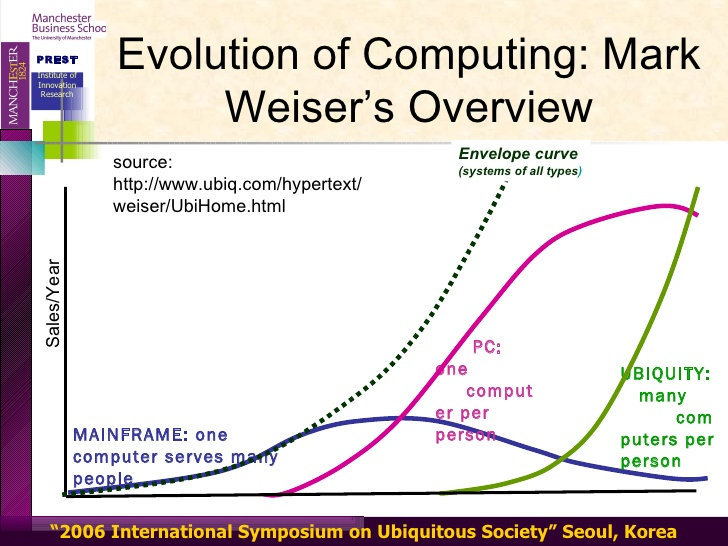
\includegraphics[width=1\textwidth]{assets/images/img1}
  \caption{Evolution of Computing: Mark Weiser's Overview}{Source: http://www.ubiq.com/hypertext/weiser/UbiHome.html (1996)} \end{figure}
%%%%%%%%%%%%%%%%%%%%%%%%%%%%%%%%%%%%%%%%%%%%%%%%%%%%%%%%%%%%%%%%%%%%Figura 01
\par The concept of pervasive computing or ubiquitous computing, exactly relates to communication devices, and how should communicate transparently to provide the user experience better. Already intelligence environments are the spaces in which embedded systems and telecommunications technologies, communicate and gather information, leading to the computing environment inserted; and all this, as said, is imperceptible to the user. Intelligence environments, currently refers to technological revolution, also known as the Internet of Things what was developed by the MIT Auto-ID Laboratory, and this type of environment is all realization of ubiquitous computing, focusing on sensioramento while computing ubiquitous focuses on communication devices.
\par This conglomerate interconnectivity is already real in our present. Today, people enjoy the technology in virtually any activity your day to day, and that's what really makes the interesting ubiquitous computing, precisely because it assist in people's lives, adapting increasingly user needs. Below is shown, according to the National Cable \& Telecommunications Association (NCTA), the advancing surge of connected devices using the Internet:
%%%%%%%%%%%%%%%%%%%%%%%%%%%%%%%%%%%%%%%%%%%%%%%%%%%%%%%%%%%%%%%%%%%%Figura 02
\begin{figure}[!ht]
  \centering
  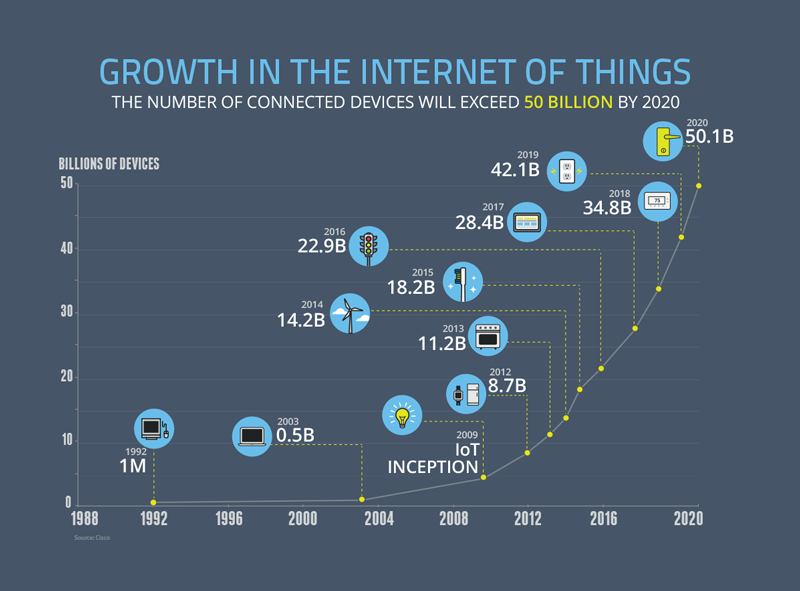
\includegraphics[width=1\textwidth]{assets/images/img2}
  \caption{Next generation Ubiquitous systems}{Source: https://www.ncta.com/platform/broadband-internet/behind-the-numbers-growth-in-the-internet-of-things/ (2015)} \end{figure}
%%%%%%%%%%%%%%%%%%%%%%%%%%%%%%%%%%%%%%%%%%%%%%%%%%%%%%%%%%%%%%%%%%%%Figura 02
\par The estimate, according to NCTA that today there are more devices connected than the quantity of human beings on planet earth. As can be seen in Figure 2, it is estimated that there will be 50 billion devices connected to 2020.Also according to the NCTA, ubiquitous Wifi and Increasing home broadband speeds quickly will drive the Internet of Things and the ever-expanding web.
%%%%%%%%%%%%%%%%%%%%%%%%%%%%%%%%%%%%%%%%%%%%%%%%%%%%%%%%%%%%%%%%%%%%%%%%%%%%%
%%%%%%%%%%%%%%%%%%%%%%%%%%%%%%%%%%%%%%%%%%%%%%%%%%%%%%%%%%%%%%%%%%%%%%%%%%%%
\section{Conclusions}
Therefore, we can conclude that ubiquitous computing is an increasing function in relation to its progressiveness, where the coordinates are the time by technology. The tecnlogias always will adapt the best way to integrate a connectivity environment, which may cause people to enjoy every day without even realizing this communication.
%%%%%%%%%%%%%%%%%%%%%%%%%%%%%%%%%%%%%%%%%%%%%%%%%%%%%%%%%%%%%%%%%%%%%%%%%%%%
%%%%%%%%%%%%%%%%%%%%%%%%%%%%%%%%%%%%%%%%%%%%%%%%%%%%%%%%%%%%%%%%%%%%%%%%%%%%
\begin{thebibliography}{00}
\bibitem{livro_mark_weiser_computacao_ubiqua} WEISER, Mark. \textbf{Some Computer Science Issues in Ubiquitous Computing.}, v. 36, n. 7, p.75-84. Communications Of The Acm, New York, jul. 1993. 
\bibitem{livro_ronzani_computação_ubiqua}Ronzani, D.(2000). \textbf{The Battle of Concepts: Ubiquitous Computing, Pervasive Computing and Ambient Intelligence in Mass Media.}
\bibitem{livro_mark_weiser_computacao_ubiqua} WEISER, Mark. \textbf{The computer for the 21 st century.} Sigmobile Mob. Comput. Commun. Rev., [s.l.], v. 3, n. 3, p.3-11, 1 jul. 1999. Association for Computing Machinery (ACM). http://dx.doi.org/10.1145/329124.329126.
\end{thebibliography}
\begin{comment}
Referencias abaixo foram geradas pelo more (mecanismo online de refencia), e este comentário possui intuito de servir como auxiliar para geração das futuras referencias deste artigo.

1º referência: WEISER, Mark. Some Computer Science Issues in Ubiquitous Computing. Communications Of The Acm, New York, v. 36, n. 7, p.75-84, jul. 1993.

Exemplos de referências montadas especificamente para o latex:
\bibitem{livro_de_c}Stroustrup, B. \textbf{The C++ Programming Language}, 4. ed. Addison-Wesley Professional, 2013.
\bibitem{livro_de_processamento_de_sinais}Oppenheim, A.V.; Schafer, R.W. \textbf{Discrete-time signal processing}. 3.ed. Prentice Hall Signal Processing, 2009. 
\end{comment}
\end{document}
